\subsection{Matched mechanism controls}
Table~\ref{tab:domain-ablation} gives a separately scheduled paired block of each complete workload. All methods use the same original questions, policy domain, cutoffs, and 16\,MiB budget. Fixed-precision controls use the primary\textquotesingle s $10^{-6}$ response tolerance. Total costs include every unresolved request; the controller includes both tiers and all retries.
\begin{table}[t]\centering\footnotesize\setlength{\tabcolsep}{2.5pt}
\caption{Matched complete-workload controls, one block per graph. Resolved coverage requires all three cutoffs of a question.}
\label{tab:domain-ablation}
\begin{tabular}{lrrrr}\toprule
&\multicolumn{2}{c}{HotpotQA}&\multicolumn{2}{c}{MuSiQue}\\
Method&Time (s)&Done (\%)&Time (s)&Done (\%)\\\midrule
ViewRank--Sparse & 149.02 & 99.70 & 169.45 & 98.97\\
NoCore & 309.31 & 22.20 & 476.09 & 16.84\\
All-row Scan & 761.84 & 99.80 & 779.80 & 98.97\\
Independent intervals & 143.02 & 46.70 & 140.28 & 52.42\\
Two-tier controller & 138.31 & 99.80 & 199.21 & 99.01\\
\bottomrule\end{tabular}\end{table}
\begin{figure}[t]\centering
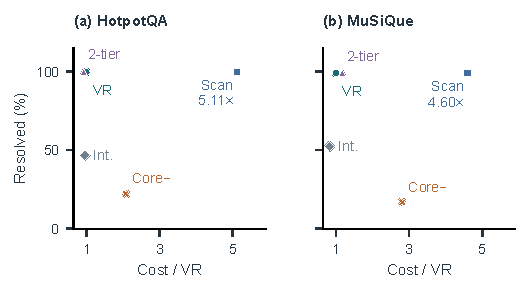
\includegraphics[width=\columnwidth]{../figures/domain_controls.pdf}
\caption{Matched component controls, one complete block per graph. VR: ViewRank; Core$-$: NoCore; Scan: all-row scan; Int.: independent intervals; 2-tier: optional controller. Cost includes all original requests and is normalized to paired VR. Read resolution jointly; Table~\ref{tab:domain-ablation} retains absolute values.}
\label{fig:domain-controls}\end{figure}
Figure~\ref{fig:domain-controls} makes the component effects visible jointly: a cheaper but unresolved workload is distinct from a complete-cost improvement at comparable or better resolution.
All-row Scan costs 5.11$\times$/4.60$\times$ VR on HotpotQA/MuSiQue with nearly identical resolution (Table~\ref{tab:domain-ablation}). NoCore changes both source coherence and its recertified posterior allowance, raising total cost while reducing completion to 222/407 questions. Independent intervals cost 4.0\%/17.2\% less but resolve only 467/1267 questions, so their saving is a cost--coverage tradeoff. The optional controller is 7.2\% faster on HotpotQA and 17.6\% slower on MuSiQue; its p95 rises to 404.3/338.7\,ms from 305.9/234.3\,ms. Fixed fine precision remains the primary.

\subsection{Certificate capacity and process memory}
Figure~\ref{fig:domain-budget} reports separate witness-free certificate-capacity runs: one paired block per graph at each budget. Success requires all three cutoffs STABLE for an original question. Tables~\ref{tab:domain-main} and~\ref{tab:domain-ablation} instead report complete three-valued audit resolution.
\begin{figure}[t]\centering
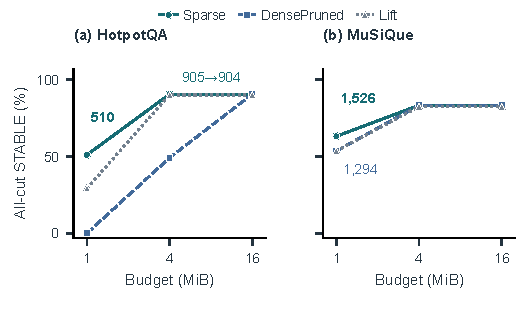
\includegraphics[width=\columnwidth]{../figures/domain_budget.pdf}
\caption{Certificate capacity at 1/4/16\,MiB: Sparse and DensePruned use the same polynomial proof; Lift uses compressed source lifting. Counts label selected points. Every original question remains in the denominator; success requires all three cutoffs \stable. Witness search is uniformly off. One block per setting; admitted numerical state is distinct from process memory.}
\label{fig:domain-budget}\end{figure}
At 1\,MiB, Sparse certifies all cutoffs for 510/1000 versus 0 for DensePruned and 293 for sparse lifting on HotpotQA; the corresponding MuSiQue counts are 1526/2417 versus 1294 for DensePruned and 1296 for sparse lifting.
At 4\,MiB, compressed retention certifies exactly the same 905 HotpotQA and 2014 MuSiQue original questions as fine DensePruned at 16\,MiB. Independent comparison confirms identical question sets and memberships at every cutoff. These are the measured configurations in Fig.~\ref{fig:domain-budget}. The Sparse HotpotQA counts are 905 at 4\,MiB and 904 at 16\,MiB; preview rows depend on cache-miss history and need not be nested across budgets. All attempted work remains charged.
\begin{table}[t]\centering\footnotesize\setlength{\tabcolsep}{2.5pt}
\caption{Fresh single-method processes, one complete run per graph at 16\,MiB with fine responses and no audit serialization. Wall is recorded producer time (seconds); peak is the cumulative process peak working set (MiB) read at block end, including the graph and backend.}
\label{tab:domain-memory}
\begin{tabular}{lrrrr}\toprule
&\multicolumn{2}{c}{HotpotQA}&\multicolumn{2}{c}{MuSiQue}\\
Method&Wall&Peak&Wall&Peak\\\midrule
ViewRank--Sparse & 140.17 & 368.8 & 117.73 & 170.1\\
DensePruned & 162.54 & 424.2 & 110.23 & 179.6\\
SourceLift, compressed & 199.81 & 356.9 & 353.26 & 166.9\\
\bottomrule\end{tabular}\end{table}
Table~\ref{tab:domain-memory} uses fresh single-method processes without audit serialization. Wall spans source freezing through execution, excluding final-summary serialization; cumulative OS working-set peaks include the graph/backend and generation scratch as well as admitted state.
